\documentclass{article}

\usepackage{graphicx}
\usepackage{tikz}
\usepackage{tikzsymbols}
\usetikzlibrary{calc,patterns,shapes.geometric}
\pagestyle{empty}
\usepackage[margin=0pt]{geometry}
\geometry{papersize={14in,12in}}

\def\centerarc[#1](#2)(#3:#4:#5){\draw[#1] ($(#2)+({#5*cos(#3)},{#5*sin(#3)})$) arc (#3:#4:#5);}

\begin{document}
	\begin{figure}
		\centering
		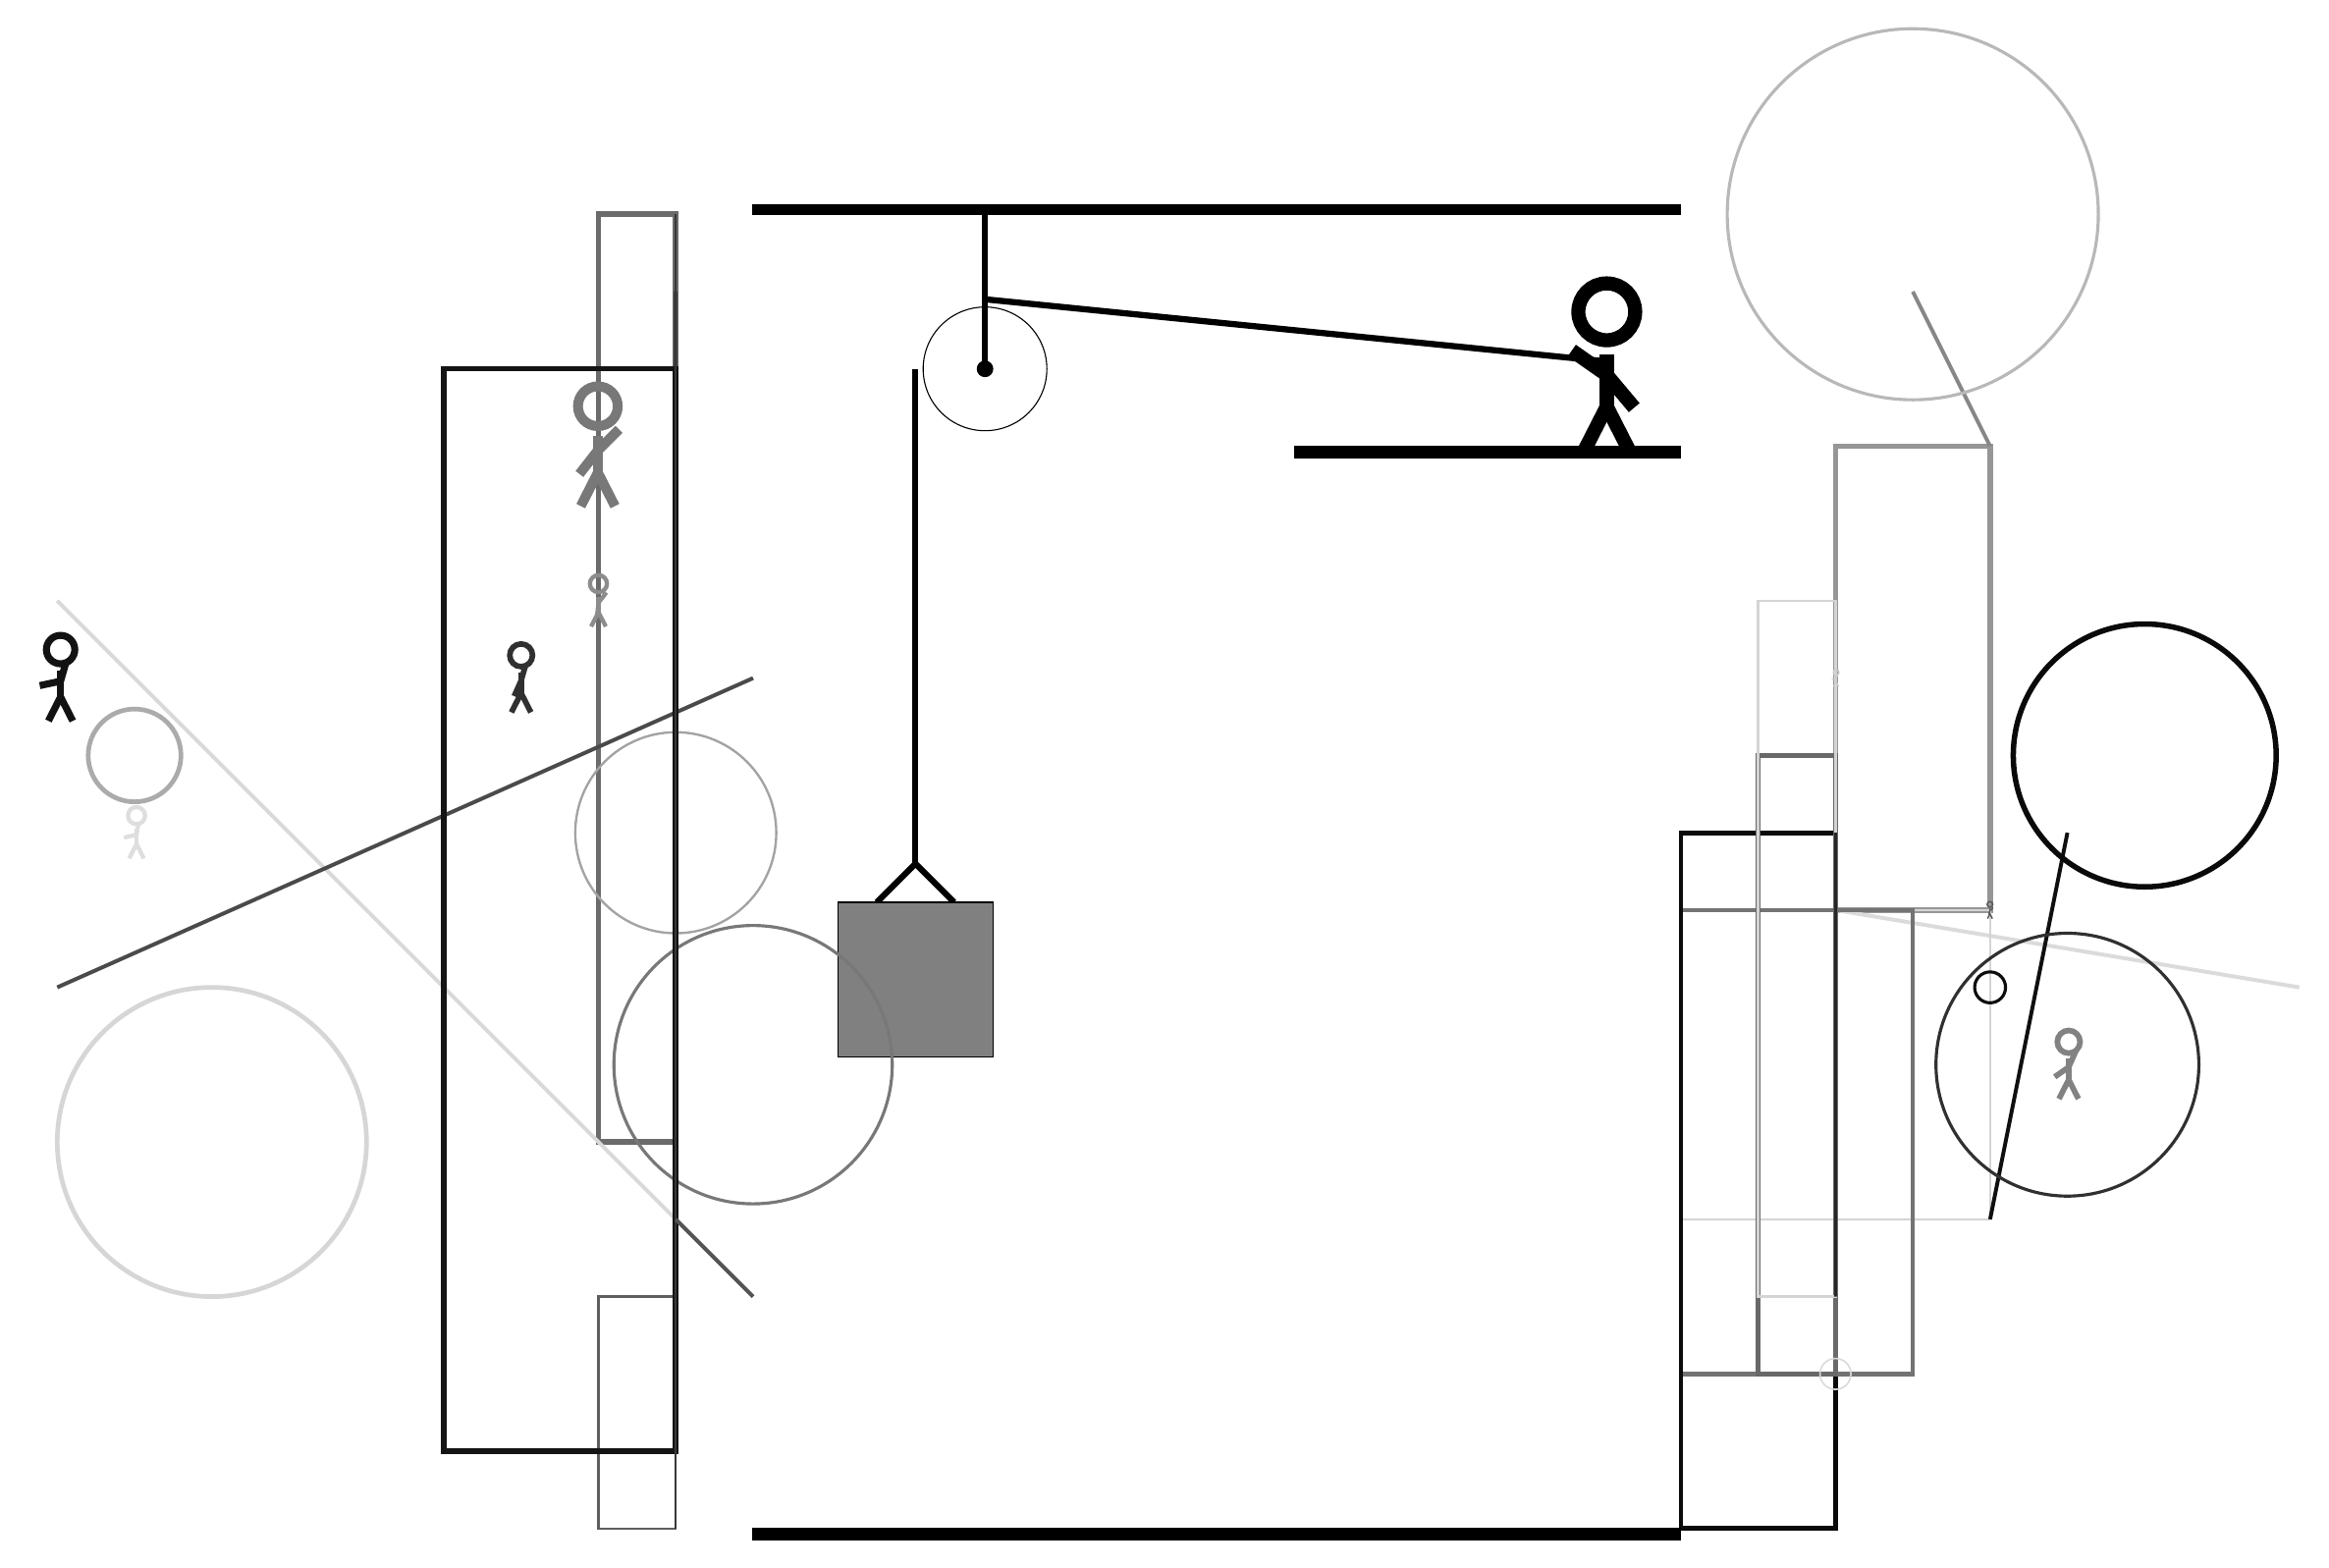
\begin{tikzpicture}
			%%%%% START %%%%%
			
			\draw[fill=black] (-2, 14) rectangle (10, 14.125);
			
			\draw (1, 12) circle (0.8);
			\draw[fill=black] (1, 12) circle (0.1);
			\draw[line width=0.8mm] (1, 14) -- (1, 12);
			
			\draw[line width=0.8mm](-0.4, 5.1) --  (0.1, 5.6) -- (0.6, 5.1);
			\draw[fill=black!50] (-0.9, 5.1) rectangle (1.1, 3.1);
			
			\draw[line width=0.8mm](0.1, 12) -- (0.1, 5.6);
			\centerarc[line width=0.8mm](1, 12)(90:180:0.9)
			\draw[line width=0.8mm](1, 12.9) -- (9, 12.1);
			
			\draw[line width=0.7mm, color=black!41] (12, 5) rectangle (14, 11);
			
			\draw[line width=0.5mm, color=black!14](12, 5) -- (18, 4);
			\draw [line width=0.6mm, color=black!16](-9, 2) circle (2.0);
			\draw[line width=0.3mm, color=black!95] (-2, 14) rectangle (-2, 14);
			
			\draw[line width=0.3mm, color=black!17] (10, 5) rectangle (14, 1);
			\draw[line width=0.7mm, color=black!58] (-3, 14) rectangle (-4, 2);
			\draw[line width=0.5mm, color=black!75] (-3, 6) rectangle (-3, 13);
			
			\draw[line width=0.5mm, color=black!15](-2, 0) -- (-11, 9);
			\draw[line width=0.6mm, color=black!55] (10, 5) rectangle (13, -1);
			
			\draw[line width=0.5mm, color=black!94](15, 6) -- (14, 1);
			\draw[line width=0.5mm, color=black!47](13, 13) -- (14, 11);
			
			\node[line width=0.4mm, color=black!13] at (-10, 6) {\Strichmaxerl[3][14][80]};
			\node[line width=0.6mm, color=black!53] at (-4, 11) {\Strichmaxerl[7][52][45]};
			\draw [line width=0.7mm, color=black!96](16, 7) circle (1.7);
			\node[line width=0.6mm, color=black!65] at (14, 5) {\Strichmaxerl[1][74][43]};
			\draw[line width=0.6mm, color=black!96] (10, -3) rectangle (12, 6);
			
			\draw[line width=0.6mm, color=black!59] (12, 7) rectangle (11, -1);
			\draw [line width=0.4mm, color=black!28](13, 14) circle (2.4);
			\draw [line width=0.4mm, color=black!81](15, 3) circle (1.7);
			\node[line width=0.7mm, color=black!49] at (15, 3) {\Strichmaxerl[4][35][66]};
			\draw[line width=0.3mm, color=black!17] (12, 9) rectangle (11, 0);
			
			\node[line width=0.5mm, color=black!45] at (-4, 9) {\Strichmaxerl[3][84][52]};
			
			\draw[line width=0.5mm, color=black!71](-2, 8) -- (-11, 4);
			\draw[line width=0.3mm, color=black!85] (12, 0) rectangle (12, 6);
			\node[line width=0.2mm, color=black!20] at (12, 8) {\Strichmaxerl[1][1][74]};
			
			\draw [line width=0.4mm, color=black!87](-9, 6) circle (0.0);
			
			\draw [line width=0.4mm, color=black!53](-2, 3) circle (1.8);
			\draw [line width=0.4mm, color=black!95](14, 4) circle (0.2);
			
			\node[line width=0.4mm, color=black!93] at (-11, 8) {\Strichmaxerl[5][12][74]};
			\draw [line width=0.3mm, color=black!36](-3, 6) circle (1.3);
			\draw[line width=0.3mm, color=black!63] (-4, 0) rectangle (-3, -3);
			
			\draw [line width=0.2mm, color=black!15](12, -1) circle (0.2);
			\draw[line width=0.7mm, color=black!92] (-3, 12) rectangle (-6, -2);
			
			\draw[line width=0.2mm, color=black!78] (-3, -3) rectangle (-3, 14);
			
			\node[line width=0.3mm, color=black!81] at (-5, 8) {\Strichmaxerl[4][66][74]};
			\draw [line width=0.6mm, color=black!33](-10, 7) circle (0.6);
			\draw[line width=0.5mm, color=black!67](-2, 0) -- (-3, 1);
			
			
			\node at (9, 12) {\Strichmaxerl[10][-35][-50]};
			\draw[fill=black] (5, 11) rectangle (10, 10.85);
			
			\draw[fill=black] (-2, -3) rectangle (10, -3.15);
			
			%%%%% END %%%%%
		\end{tikzpicture}
	\end{figure}	
\end{document}